\chapter{Kết quả chi tiết và tái lập}
\section{Audit huấn luyện E1--E3}
Các bảng dưới ghi số epoch đã chạy, best epoch, optimizer updates thực tế,
AMP skips và peak allocated MiB. Chúng đối chiếu trực tiếp output cell,
không suy số updates chỉ từ số epoch.
\DataTable{assets/e1/audit.tex}{Audit E1.}
\DataTable{assets/e2/audit.tex}{Audit E2; ký hiệu M/T và R/P/C như Chương E2.}
\DataTable{assets/e3/audit.tex}{Audit E3.}
\DataTable{assets/a1/extended_cost.tex}{Epoch, cập nhật và peak memory của sáu run mở rộng A1.}
\section{Metric theo lớp và độ nhạy A1}
Hai cột model là full pretrained seed 42, được chọn bằng validation.
Support là số ảnh test nguồn. ID tra bằng bảng tên lớp dưới đây.

\DataTable{assets/a1/perclass_1.tex}{Precision/recall/F1 trên test GTSRB, lớp 0--21.}
\DataTable{assets/a1/perclass_2.tex}{Precision/recall/F1 trên test GTSRB, lớp 22--42.}

\begin{table}[H]\centering\caption{Độ nhạy A1 với 8 ảnh test trùng train.}
\small\begin{tabular}{lrrrrr}\toprule Run & Full acc & Clean acc & $\Delta$ (điểm\%) & Full F1 & Clean F1\\\midrule
R-S/42 & 96.33 & 96.33 & -0.002 & 0.9447 & 0.9447\\
R-H/42 & 70.35 & 70.33 & -0.019 & 0.6143 & 0.6143\\
R-P/42 & 96.05 & 96.05 & -0.003 & 0.9438 & 0.9438\\
R-F/42 & 98.37 & 98.37 & -0.001 & 0.9743 & 0.9743\\
D-S/42 & 96.14 & 96.13 & -0.002 & 0.9350 & 0.9350\\
D-H/42 & 69.73 & 69.71 & -0.019 & 0.6125 & 0.6125\\
D-P/42 & 87.85 & 87.85 & -0.008 & 0.8063 & 0.8063\\
D-F/42 & 98.92 & 98.91 & -0.001 & 0.9790 & 0.9790\\

\bottomrule\end{tabular}\end{table}
Full test có 12.630 ảnh, clean test có 12.622; mọi accuracy là\%.
Bảng ghi mức làm tròn trong output; delta tính trên giá trị chưa làm tròn nên
không nhất thiết bằng phép trừ hai cột accuracy hiển thị.

\begin{landscape}
\section{Ma trận nhầm lẫn E2 và E3}
Mỗi cặp dùng cùng thang màu 0--100\%, ghi cả count và tỷ lệ theo hàng.
Toàn bộ 10.000 ảnh test mỗi model được đưa vào ma trận. Các model không được
chọn/tune lại theo lỗi test ở các hình này.
\begin{figure}[H]\centering
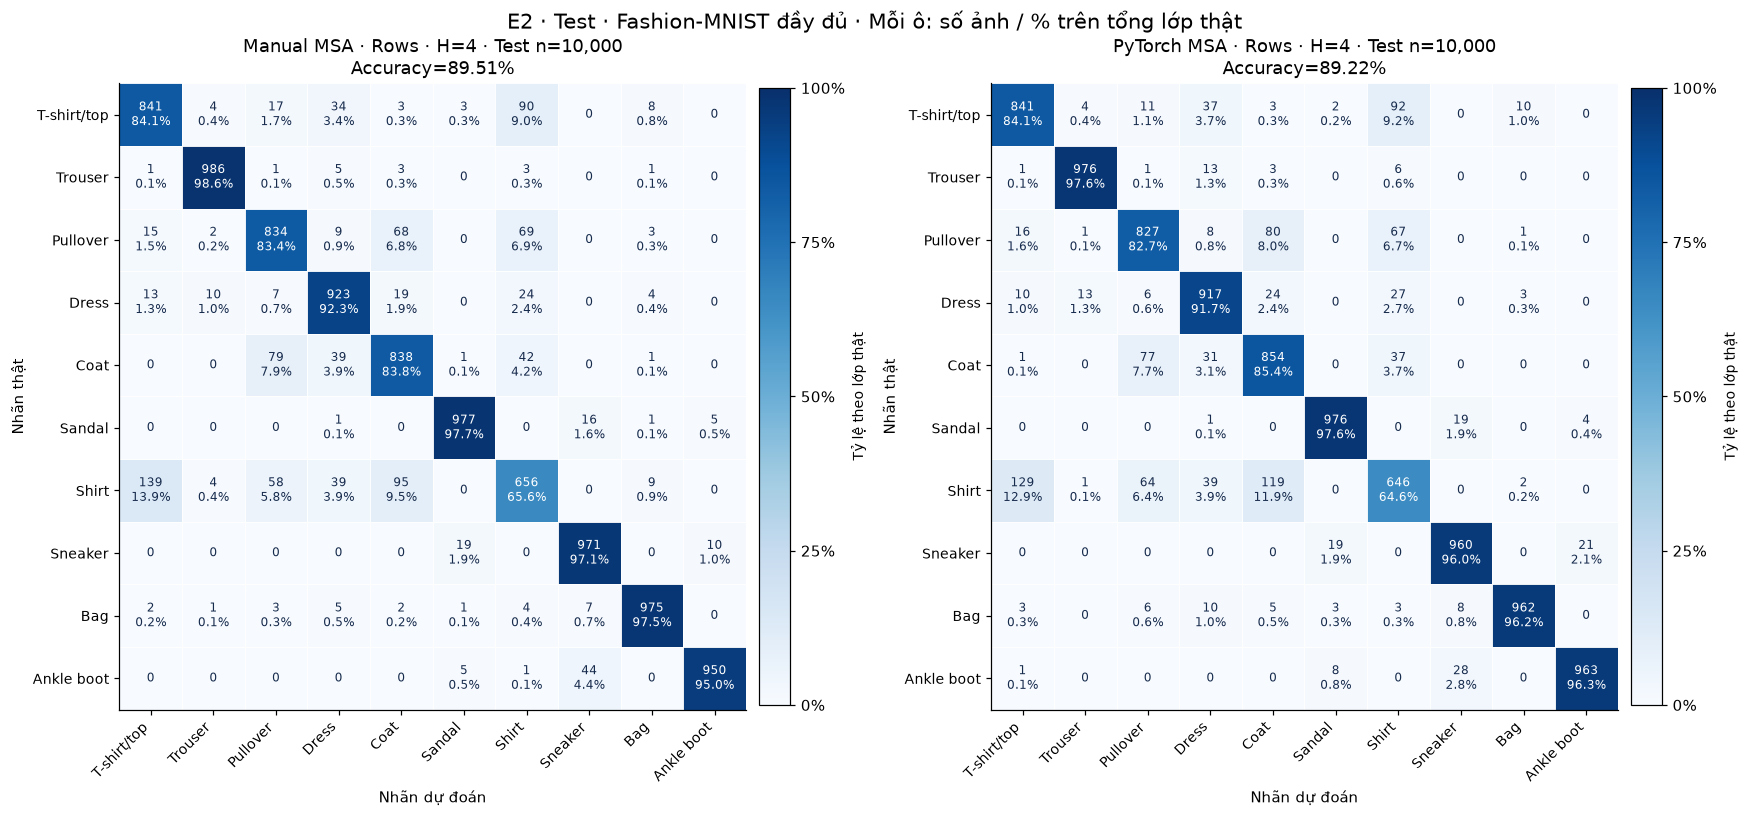
\includegraphics[width=.98\linewidth,height=.67\textheight,keepaspectratio]{assets/e2/confusion_test_pair_1.png}
\caption{E2: confusion matrix test, cặp1; tên model ghi trên từng panel.}\end{figure}\end{landscape}
\begin{landscape}\begin{figure}[p]\centering
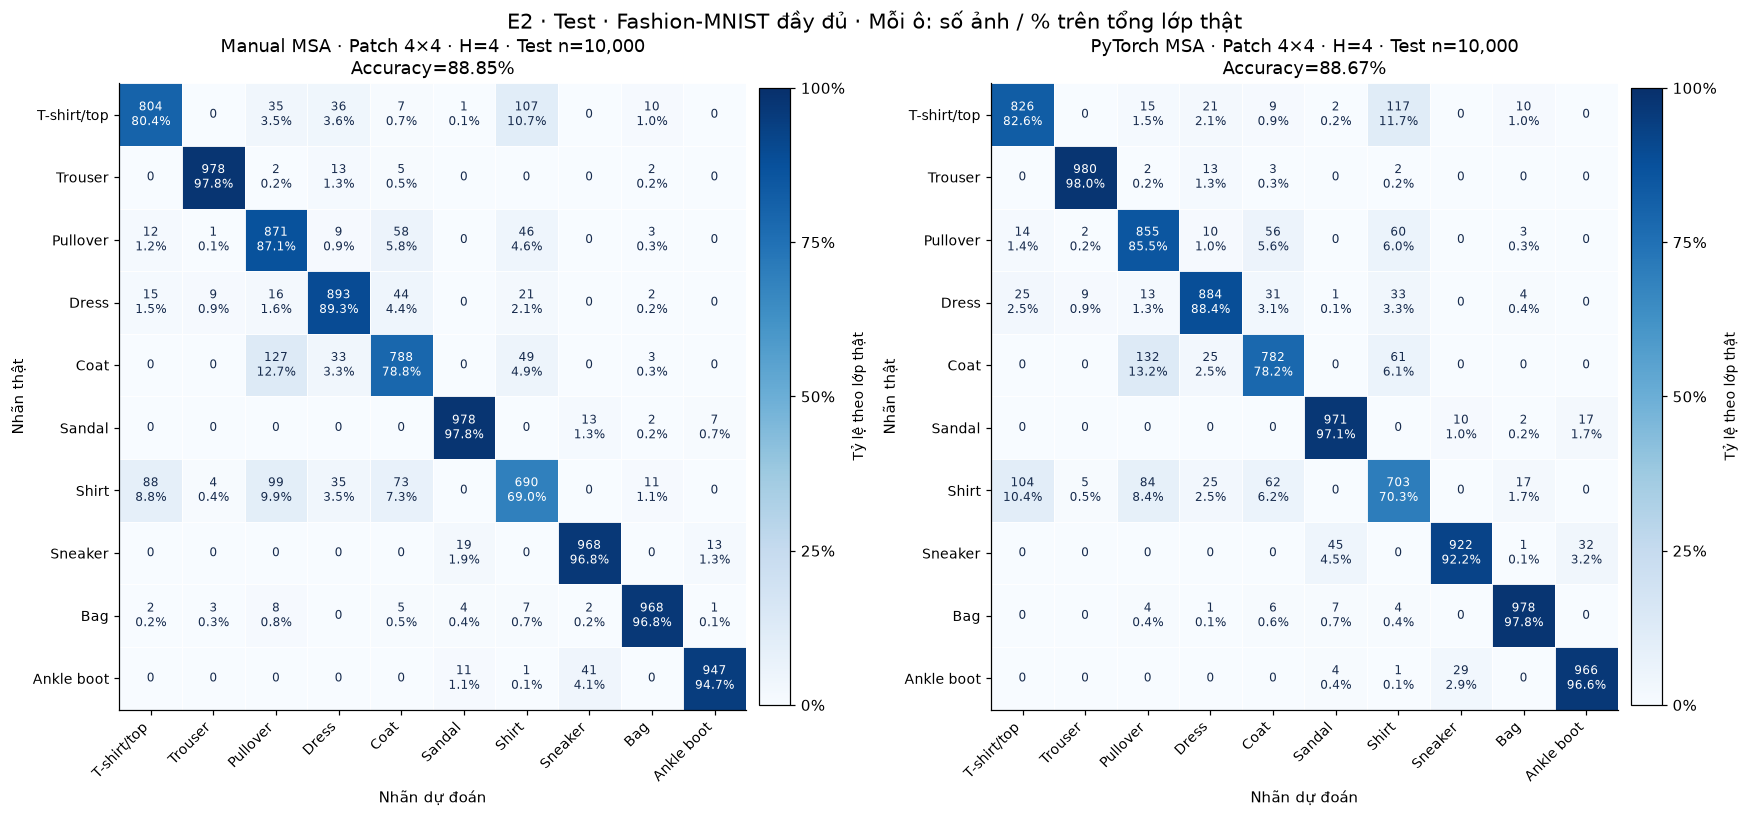
\includegraphics[width=.98\linewidth,height=.86\textheight,keepaspectratio]{assets/e2/confusion_test_pair_2.png}
\caption{E2: confusion matrix test, cặp2; tên model ghi trên từng panel.}\end{figure}\end{landscape}
\begin{landscape}\begin{figure}[p]\centering
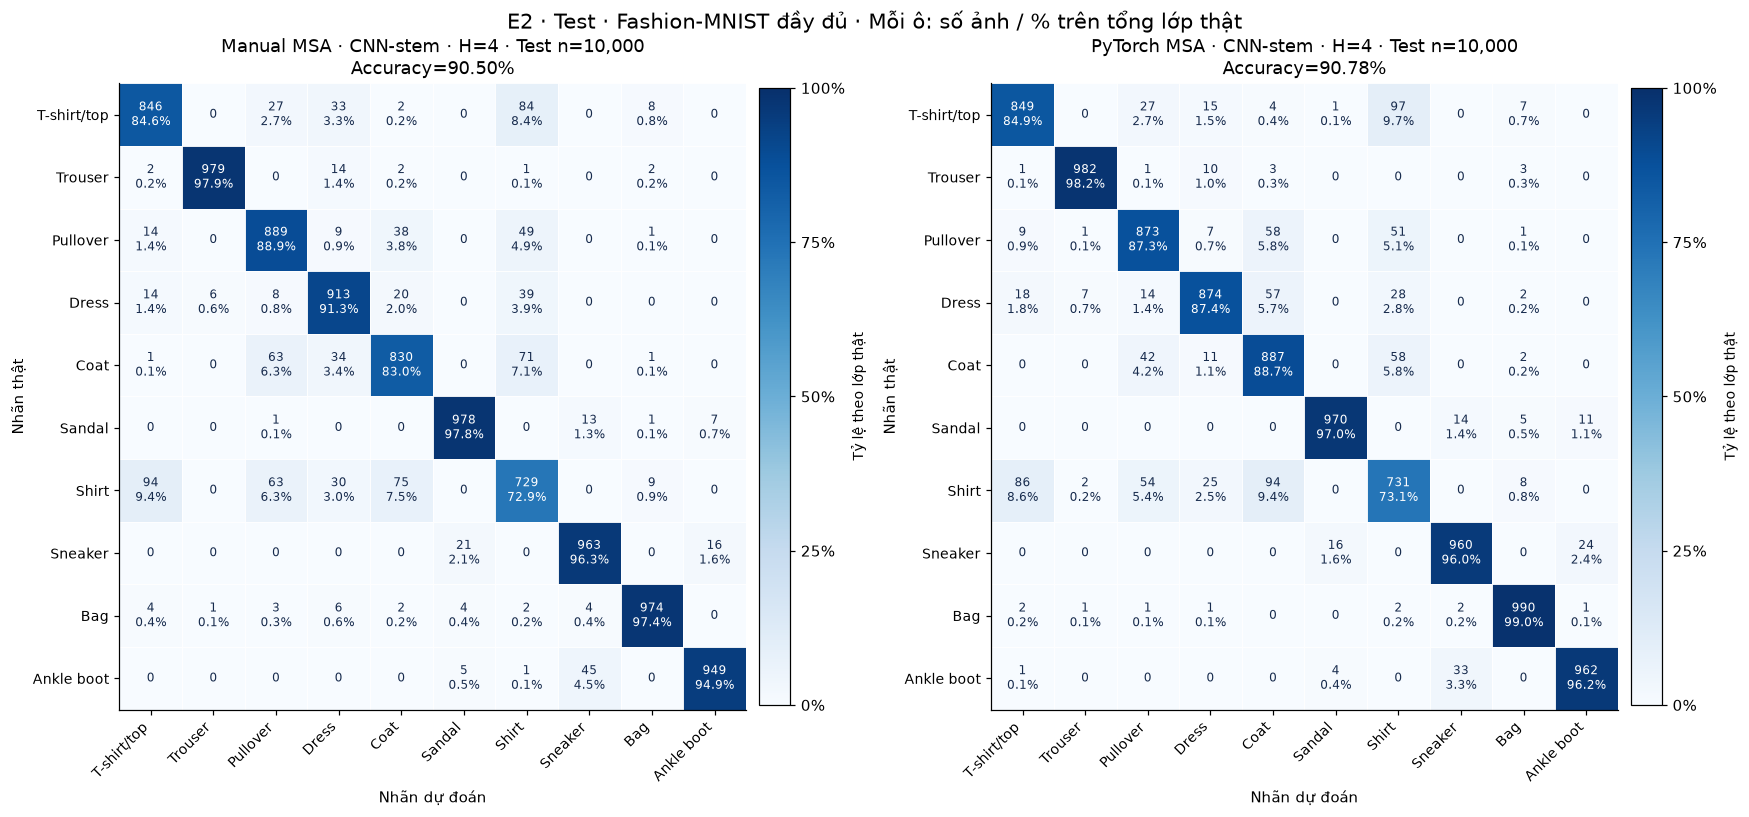
\includegraphics[width=.98\linewidth,height=.86\textheight,keepaspectratio]{assets/e2/confusion_test_pair_3.png}
\caption{E2: confusion matrix test, cặp3; tên model ghi trên từng panel.}\end{figure}\end{landscape}
\begin{landscape}\begin{figure}[p]\centering
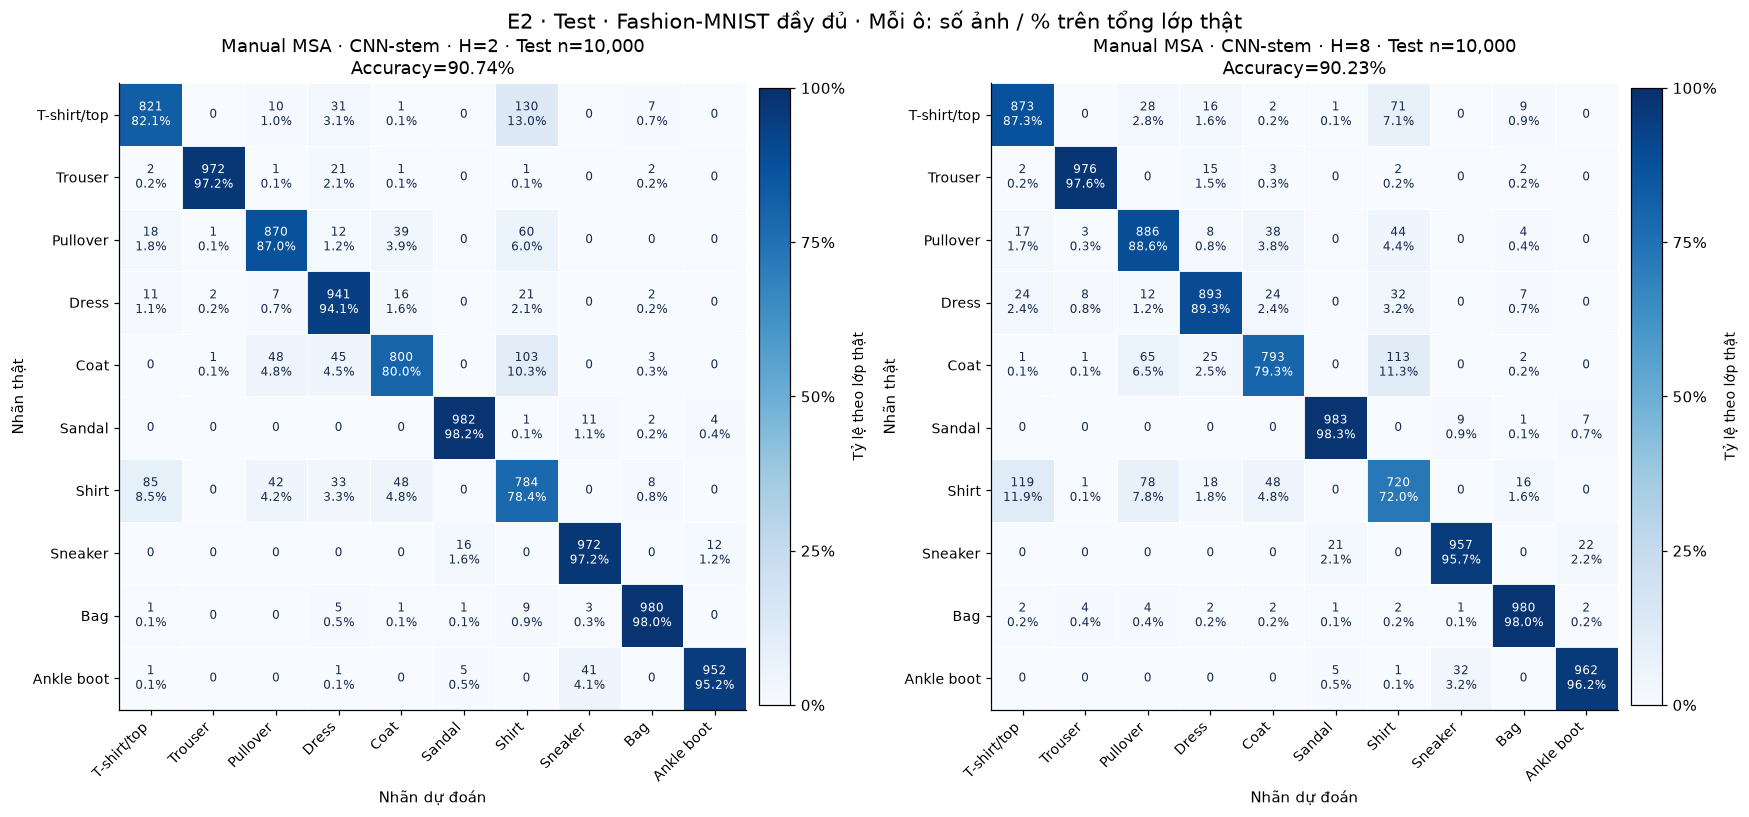
\includegraphics[width=.98\linewidth,height=.86\textheight,keepaspectratio]{assets/e2/confusion_test_pair_4.png}
\caption{E2: confusion matrix test, cặp4; tên model ghi trên từng panel.}\end{figure}\end{landscape}
\begin{landscape}\begin{figure}[p]\centering
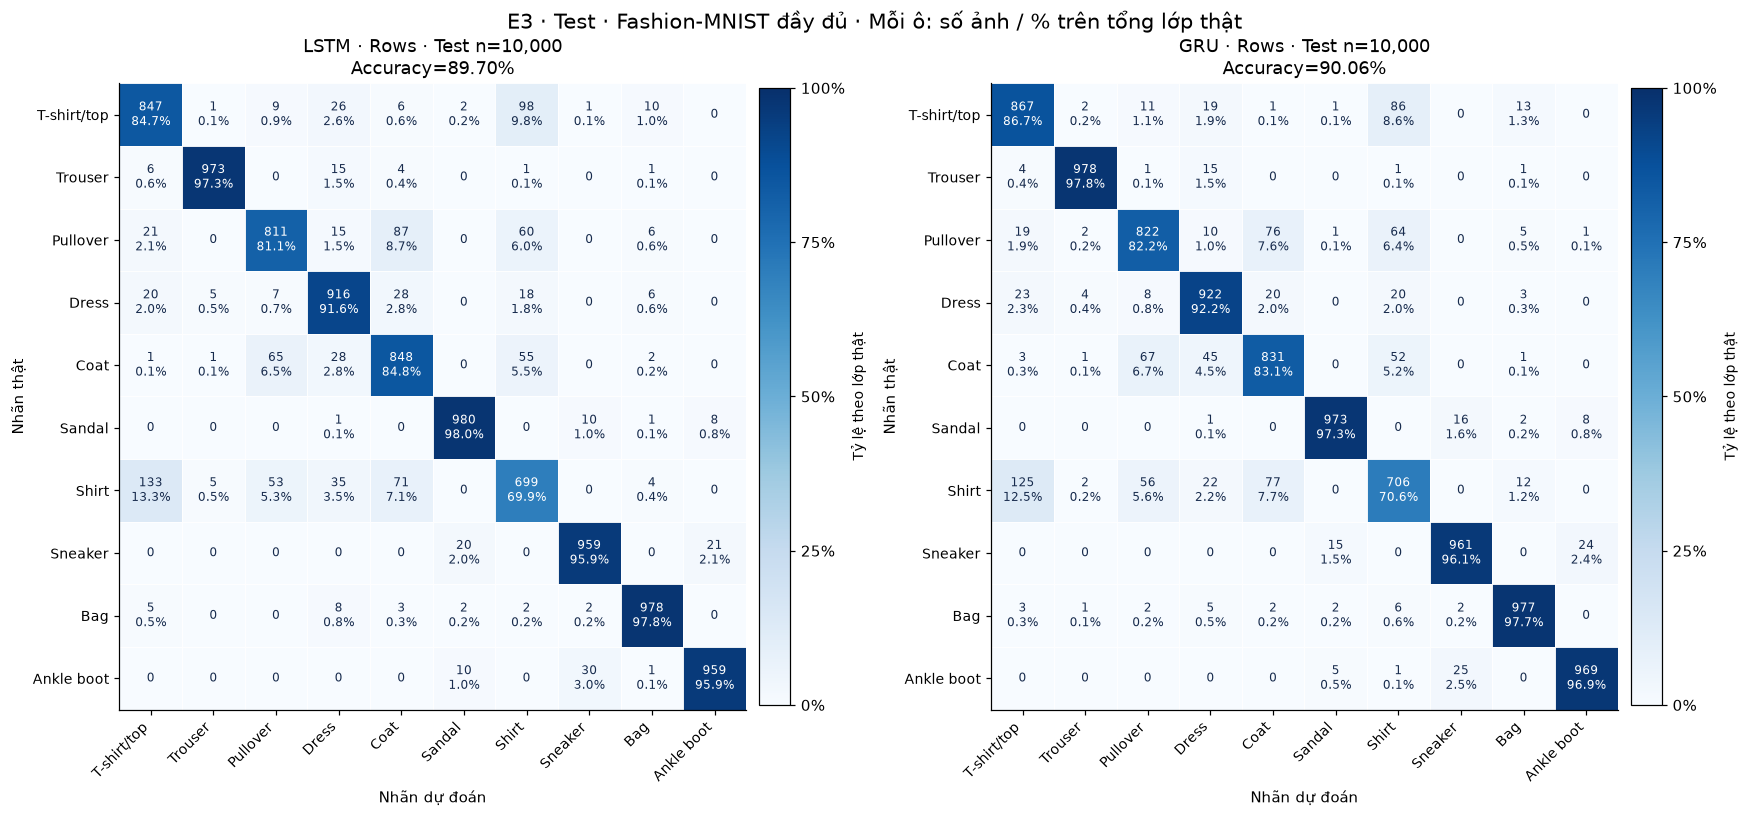
\includegraphics[width=.98\linewidth,height=.86\textheight,keepaspectratio]{assets/e3/confusion_test_pair_1.png}
\caption{E3: confusion matrix test, cặp1; tên model ghi trên từng panel.}\end{figure}\end{landscape}
\begin{landscape}\begin{figure}[p]\centering
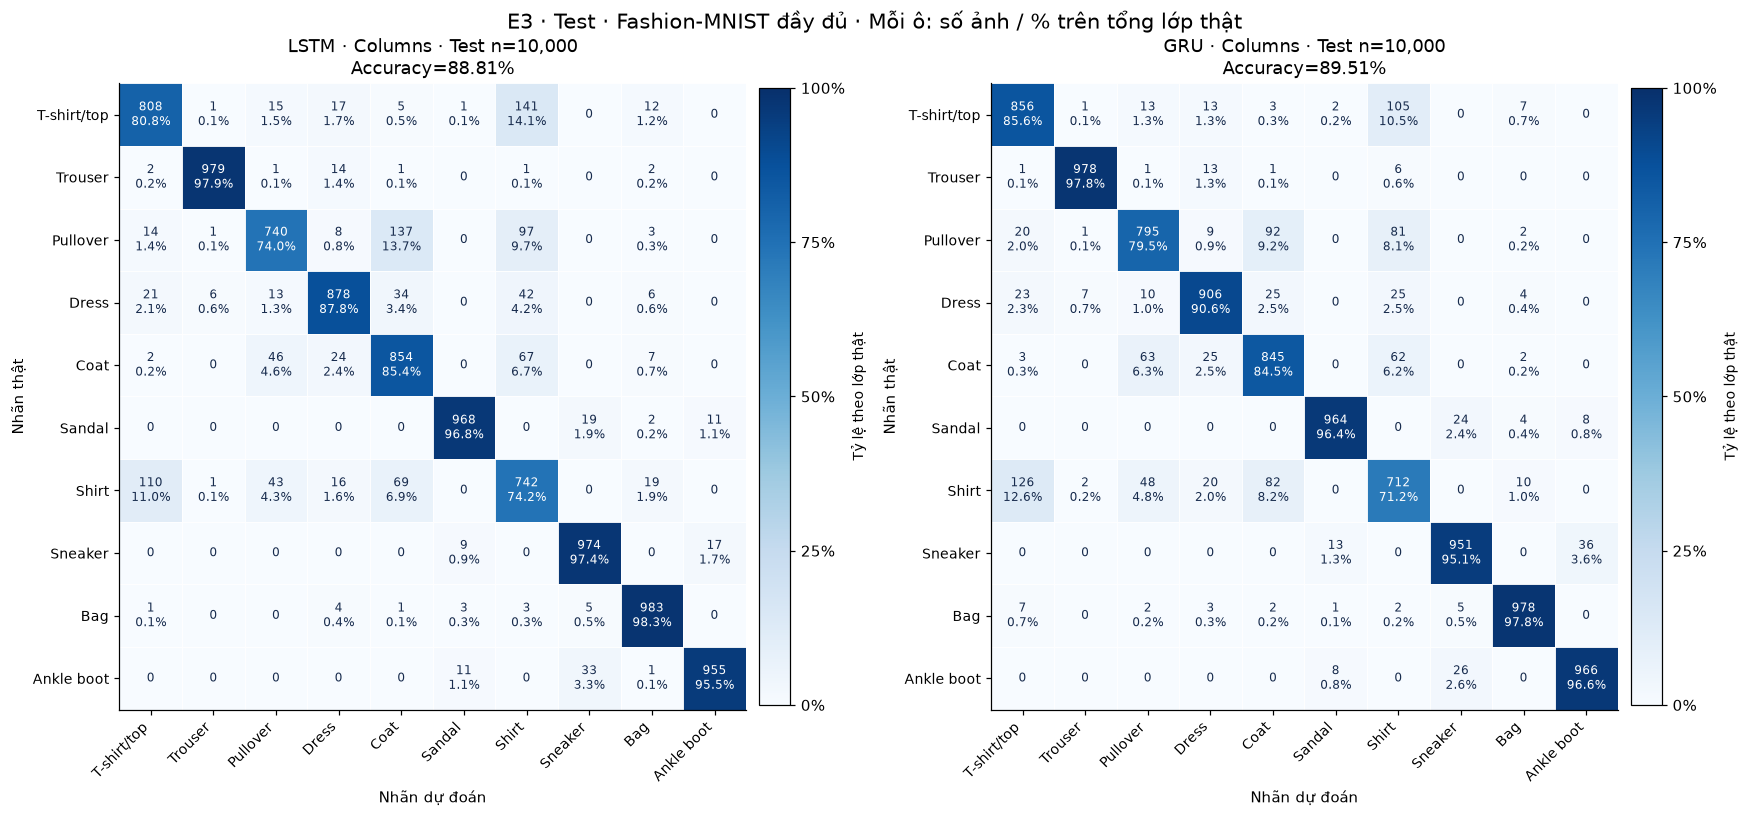
\includegraphics[width=.98\linewidth,height=.86\textheight,keepaspectratio]{assets/e3/confusion_test_pair_2.png}
\caption{E3: confusion matrix test, cặp2; tên model ghi trên từng panel.}\end{figure}\end{landscape}
\begin{landscape}\begin{figure}[p]\centering
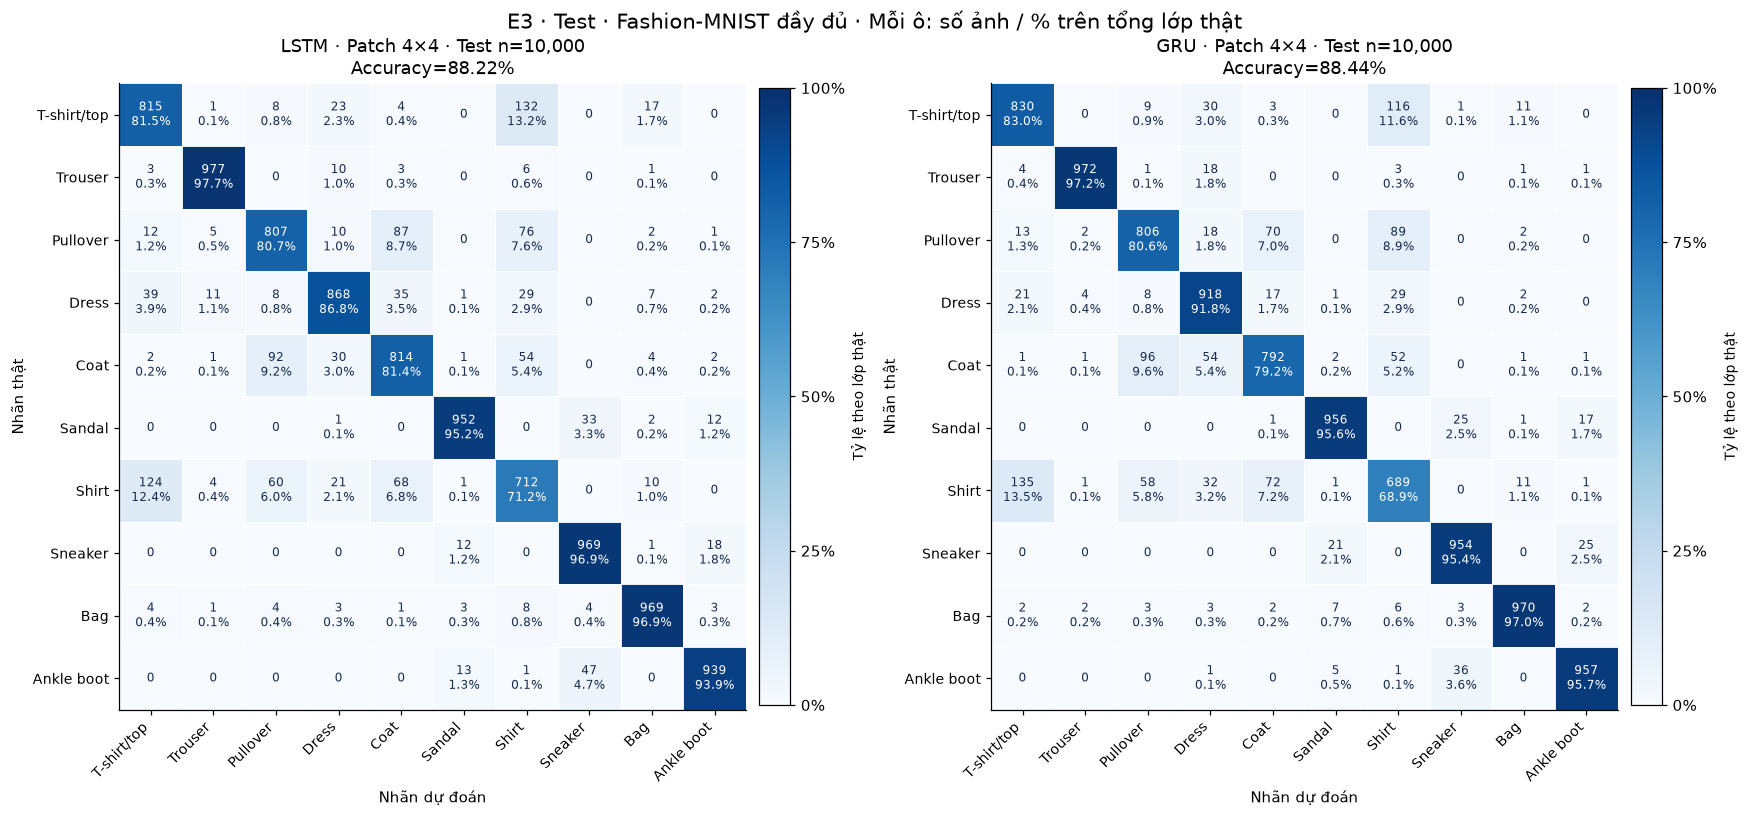
\includegraphics[width=.98\linewidth,height=.86\textheight,keepaspectratio]{assets/e3/confusion_test_pair_3.png}
\caption{E3: confusion matrix test, cặp3; tên model ghi trên từng panel.}\end{figure}\end{landscape}
\begin{landscape}\begin{figure}[p]\centering
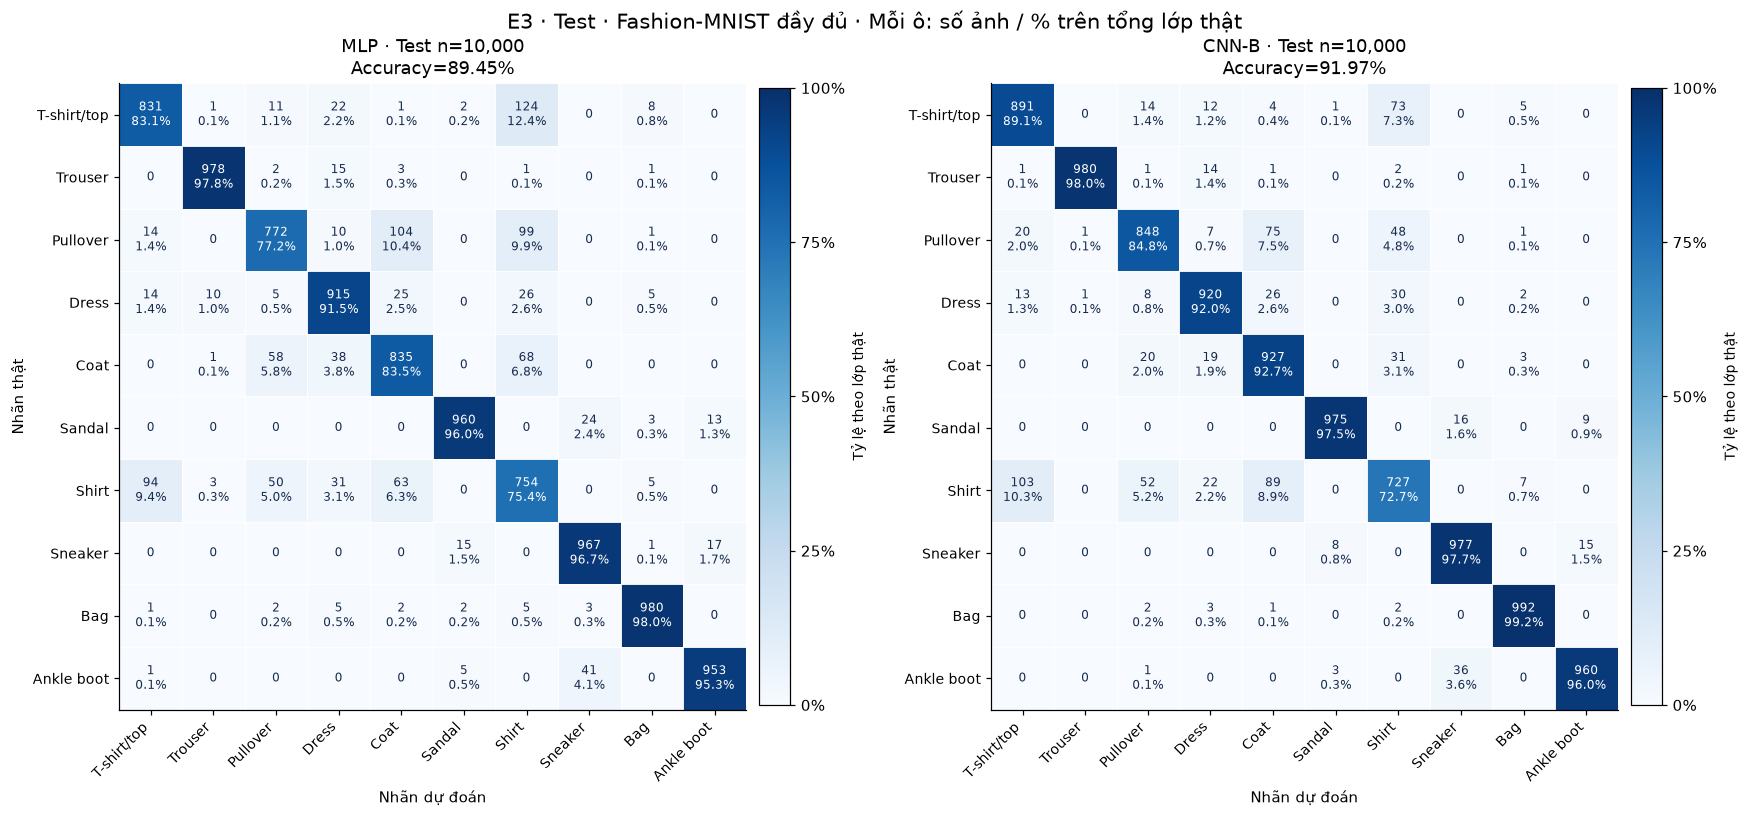
\includegraphics[width=.98\linewidth,height=.86\textheight,keepaspectratio]{assets/e3/confusion_test_pair_4.png}
\caption{E3: confusion matrix test, cặp4; tên model ghi trên từng panel.}\end{figure}\end{landscape}

\section{Nguồn số liệu và hướng dẫn tái lập}
Nguồn số liệu là output đã lưu của E1.ipynb, E2.ipynb, E3.ipynb và A1.ipynb
trong source\_code. Manifest dưới assets/e1, e2, e3, a1 ghi cell/output và
bảng Markdown nguồn; PNG trích từ ảnh embedded trong notebook, không chạy
training để tạo lại số liệu. Notebook không tự ghi assets của báo cáo.

Chuẩn bị dữ liệu theo README trong thư mục datasets. Mở notebook tương ứng,
chọn Python 3.14 có CUDA, Restart Kernel và Run All, sau đó Save. Mỗi notebook
chạy độc lập; không cần thứ tự. Để tái hiện đúng số liệu lịch sử E1--E3,
cần dùng cấu hình patience10 ghi trong output; mặc định code hiện tại là 4.
A1 sử dụng patience 4 như số liệu đã báo cáo. Seed cố định không đảm bảo
tái lập bitwise qua mọi GPU, phiên bản thư viện hoặc đường thực thi AMP.

Báo cáo biên dịch bằng XeLaTeX và BibTeX từ report/source\_latex/main.tex;
các sơ đồ kiến trúc là mã TikZ trong từng chương, ảnh kết quả nằm ở assets.
Sản phẩm PDF chung giữ tại report/CO5085\_Report.pdf.
